Im Rahmen des Praktikums wurde zuerst der Datensatz analysiert. Im Folgenden wird zunächst der ursprüngliche Datensatz beschrieben und anschließend erklärt, wie dieser im Laufe des Projekts ausgebaut und ergänzt wird. Danach wird die daraus abgeleitete Problemstellung erläutert.

\subsection{Ursprünglicher Datensatz}
\label{UrsprunglicherDatensatz}
Als Basis wurde der Datensatz \cite{Urbanbricks2020} verwendet, welcher sowohl hochwertige Wikipediaeinträge enthält, die den Status eines \emph{Good Article} erreicht haben, sowie Artikel mit \textit{promotional} (werblichen) Inhalten. Ein \emph{Good Article} erf"ullt bestimmte Qualitätskriterien wie eine verständliche Schreibweise, faktische Korrektheit und Neutralität \cite{WikiGA}. Diese Artikel haben den Begutachtungsprozess der Wikipedia erfolgreich durchlaufen. Die werblichen Artikel sind in verschiedene Kategorien unterteilt: \emph{advert} (klassische Werbeanzeigen), \emph{coi} (Interessenkonflikte des Autors), \emph{fanpov} (mögliche Fandarstellung), \emph{PR} (Presseartikel) und \emph{resume} (Lebensläufe).

Der Datensatz zeigte erhebliche Ungleichgewichte in der Verteilung der Werbe-Labels.

\begin{figure}[H]
    \centering
    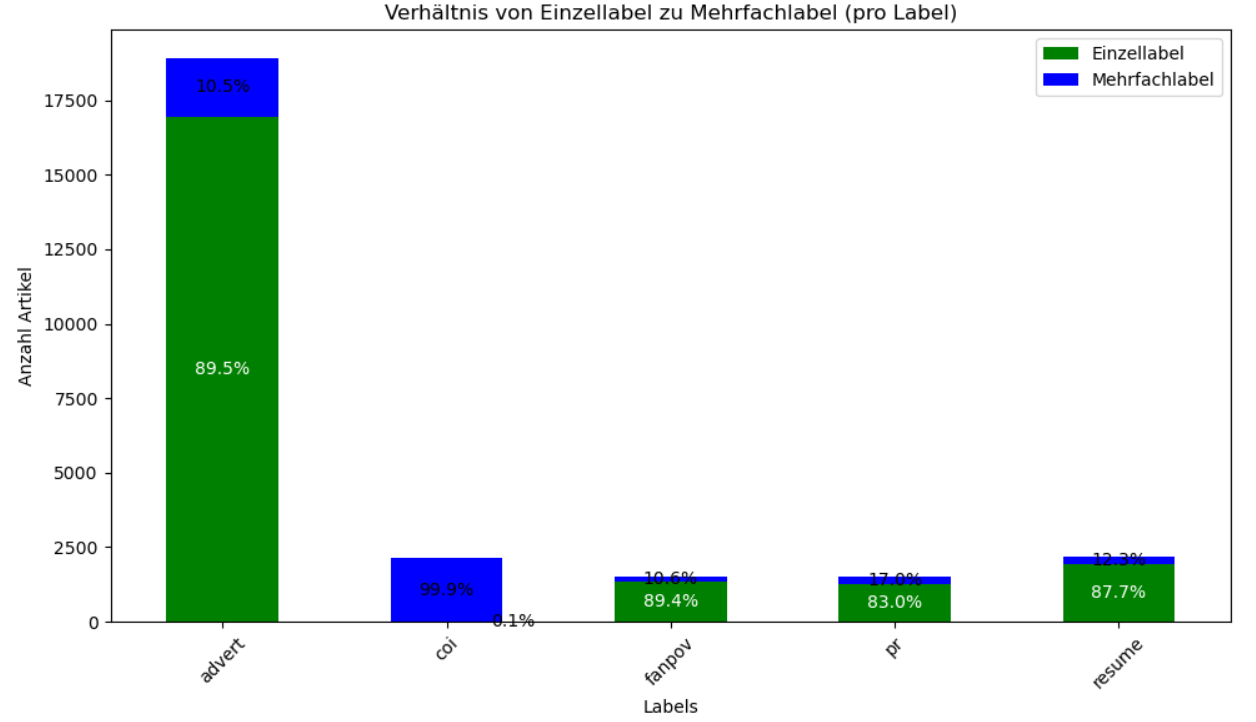
\includegraphics[width=0.7\linewidth]{figures/labelverteilung.png}
    \caption{Verteilung der Werbelabels.}
    \label{fig:labelverteilung}
\end{figure}

Wie in Abbildung \ref{fig:labelverteilung} deutlich wird, dominiert das Label advert gegenüber den anderen Labels, während insbesondere coi mit nur drei eigenständigen Labels stark unterrepräsentiert ist. Dies birgt die Gefahr, dass Modelle Schwierigkeiten haben, die weniger häufigen Werbe-Labels korrekt zu erkennen.
\subsection{Datensatzerweiterung}
\label{ProblemeDatensatz}
\label{WPDump}
Aufgrund der beschriebenen Herausforderungen mit dem Datensatz von Kaggle, wurden weitere Artikel mittels Wikipedia-Dump beschafft. Beim Wikipedia-Dump handelt es sich um einen von der Wikimedia-Foundation veröffentlichten Datensatz, der alle Wikipedia-Seiten umfasst. Der Dump der englischsprachigen Wikipedia ist unter \cite{WpDump2024} zu finden.

Da die Seiten im Dump in Wiki-Syntax vorliegen, enthalten sie auch alle von den Wikipedia-Autoren eingesetzten Vorlagen (Templates). Jeder Artikel, der von der Wiki\-pedia-Gemeinschaft als lesenswert (\emph{good}), exzellent (\emph{featured}) oder werbend (\emph{promotional}) klassifiziert wurde, enthält mindestens ein Template, anhand dessen diese Klassifizierung erkannt werden kann. Außerdem lassen sich anhand von Templates und anderen Syntax-Elementen noch diejenigen Seiten identifizieren, welche keine Artikel darstellen, beispielsweise Begriffsklärungsseiten, Umleitungen, Kategorien und Benutzerseiten.

Es wurde ein Konverter entwickelt, der die Artikel anhand der Templates auf drei Kategorien verteilt und in CSV-Dateien schreibt: In die erste Kategorie \emph{good} fallen die als lesenswert und exzellent gekennzeichneten; in die zweite Kategorie \emph{promotional} die als werbend erkannten und in die letzte Kategorie \emph{neutral} alle weiteren Artikel. Die zur Kategorisierung genutzten Templates wurden aus dem Artikeltext entfernt. Insgesamt ergab sich die folgende Aufteilung: 46.882 \emph{good}, 32.633 \emph{promotional}, 6.611.303 \emph{neutral}. Da die Klassen extrem ungleich verteilt sind, wurde anschließend noch eine gleichgroße zufällige Auswahl der Artikel jeder Klasse getroffen (Undersampling). Hierbei kam \textit{Reservoir Sampling} \cite{Vitter1985} zum Einsatz, bei dem die Elemente des Datensatzes einzeln gelesen werden, ohne dass deren Anzahl zuvor bekannt sein muss.

\subsection{Problemdefinition}
\label{Problemdefinition}
Das Ziel dieses Projekts ist die Entwicklung von Modellen zur automatisierten Klassifikation von Wikipedia-Artikeln hinsichtlich ihres \textit{promotional} (werblichen) Charakters. Dabei haben wir uns mit den folgenden zwei Fragestellungen beschäftigt:
\begin{enumerate}
    \item Ist ein gegebener Wikipedia-Artikel promotional oder nicht-promotional?

    \item Falls ein Wikipedia-Artikel als promotional klassifiziert wurde, welche Label treffen auf ihn zu?
\end{enumerate}
